\documentclass[a4paper]{report}
\usepackage[utf8]{inputenc}
\usepackage[T1]{fontenc}
\usepackage{textcomp}

\usepackage{url}

\usepackage{hyperref}
\hypersetup{
    colorlinks,
    linkcolor={black},
    citecolor={black},
    urlcolor={blue!80!black}
}

\usepackage{graphicx}
\usepackage{wrapfig}
\usepackage{adjustbox}
\usepackage{float}
\usepackage[usenames,dvipsnames]{xcolor}

\usepackage{listings}

\lstset{
    language=Python,
    basicstyle=\ttfamily\footnotesize,
    keywordstyle=\color{blue},
    stringstyle=\color{red},
    commentstyle=\color{gray},
    showstringspaces=false,
    frame=single,
    numbers=left,
    numberstyle=\tiny,
    breaklines=true,
    tabsize=4
}

% \usepackage{cmbright}

\usepackage{amsmath, amsfonts, mathtools, amsthm, amssymb}
\usepackage{mathrsfs}
\usepackage{cancel}

\newcommand\N{\ensuremath{\mathbb{N}}}
\newcommand\R{\ensuremath{\mathbb{R}}}
\newcommand\Z{\ensuremath{\mathbb{Z}}}
\renewcommand\O{\ensuremath{\emptyset}}
\newcommand\Q{\ensuremath{\mathbb{Q}}}
\newcommand\C{\ensuremath{\mathbb{C}}}
\let\implies\Rightarrow
\let\impliedby\Leftarrow
\let\iff\Leftrightarrow
\let\epsilon\varepsilon

% horizontal rule
\newcommand\hr{
    \noindent\rule[0.5ex]{\linewidth}{0.5pt}
}

\usepackage{tikz}
% \usepackage{tikzmark}
\usepackage{pgfplots}
\usepackage{tikz-cd}

\usetikzlibrary{calc, arrows.meta, positioning, angles, quotes, patterns}

% theorems
\usepackage{thmtools}
\usepackage{thm-restate}
\usepackage[framemethod=TikZ]{mdframed}
\mdfsetup{skipabove=1em,skipbelow=0em, innertopmargin=12pt, innerbottommargin=8pt}

\theoremstyle{definition}

\makeatletter

\declaretheoremstyle[
    headfont=\bfseries\sffamily\color{ForestGreen!70!black}, bodyfont=\normalfont,
    mdframed={
        linewidth=2pt,
        rightline=false, topline=false, bottomline=false,
        linecolor=ForestGreen, backgroundcolor=ForestGreen!5,
    }
]{thmgreenbox}

\declaretheoremstyle[
    headfont=\bfseries\sffamily\color{NavyBlue!70!black}, bodyfont=\normalfont,
    mdframed={
        linewidth=2pt,
        rightline=false, topline=false, bottomline=false,
        linecolor=NavyBlue, backgroundcolor=NavyBlue!5,
    }
]{thmbluebox}

\declaretheoremstyle[
    headfont=\bfseries\sffamily\color{NavyBlue!70!black}, bodyfont=\normalfont,
    mdframed={
        linewidth=2pt,
        rightline=false, topline=false, bottomline=false,
        linecolor=NavyBlue
    }
]{thmblueline}

\declaretheoremstyle[
    headfont=\bfseries\sffamily\color{RawSienna!70!black}, bodyfont=\normalfont,
    mdframed={
        linewidth=2pt,
        rightline=false, topline=false, bottomline=false,
        linecolor=RawSienna, backgroundcolor=RawSienna!5,
    }
]{thmredbox}

\declaretheoremstyle[
    headfont=\bfseries\sffamily\color{RawSienna!70!black}, bodyfont=\normalfont,
    numbered=no,
    mdframed={
        linewidth=2pt,
        rightline=false, topline=false, bottomline=false,
        linecolor=RawSienna, backgroundcolor=RawSienna!1,
    },
    qed=\qedsymbol
]{thmproofbox}

\declaretheoremstyle[
    headfont=\bfseries\sffamily\color{NavyBlue!70!black}, bodyfont=\normalfont,
    numbered=no,
    mdframed={
        linewidth=2pt,
        rightline=false, topline=false, bottomline=false,
        linecolor=NavyBlue, backgroundcolor=NavyBlue!1,
    },
]{thmexplanationbox}

\declaretheorem[numberwithin=chapter, style=thmgreenbox, name=Definition]{definition}
\declaretheorem[sibling=definition, style=thmredbox, name=Corollary]{corollary}
\declaretheorem[sibling=definition, style=thmredbox, name=Proposition]{prop}
\declaretheorem[sibling=definition, style=thmredbox, name=Theorem]{theorem}
\declaretheorem[sibling=definition, style=thmredbox, name=Lemma]{lemma}
\declaretheorem[sibling=definition, style=thmbluebox,  name=Example]{eg}
\declaretheorem[sibling=definition, style=thmbluebox,  name=Nonexample]{noneg}
\declaretheorem[sibling=definition, style=thmblueline, name=Remark]{remark}




\declaretheorem[numbered=no, style=thmexplanationbox, name=Proof]{explanation}
\declaretheorem[numbered=no, style=thmproofbox, name=Proof]{preuve}
\declaretheorem[style=thmbluebox,  numbered=no, name=Exercise]{ex}
\declaretheorem[style=thmblueline, numbered=no, name=Note]{note}

% \renewenvironment{proof}[1][\proofname]{\begin{replacementproof}}{\end{replacementproof}}

% \AtEndEnvironment{eg}{\null\hfill$\diamond$}%

\newtheorem*{uovt}{UOVT}
\newtheorem*{notation}{Notation}
\newtheorem*{previouslyseen}{As previously seen}
\newtheorem*{problem}{Problem}
\newtheorem*{observe}{Observe}
\newtheorem*{property}{Property}
\newtheorem*{intuition}{Intuition}


\declaretheoremstyle[
    headfont=\bfseries\sffamily\color{RawSienna!70!black}, bodyfont=\normalfont,
    mdframed={
        linewidth=2pt,
        rightline=false, topline=false, bottomline=false,
        linecolor=RawSienna, backgroundcolor=RawSienna!5,
    }
]{todo}
\declaretheorem[numbered=no, style=todo, name=TODO]{TODO}


\usepackage{etoolbox}

\AtEndEnvironment{vb}{\null\hfill$\diamond$}%
\AtEndEnvironment{intermezzo}{\null\hfill$\diamond$}%




% http://tex.stackexchange.com/questions/22119/how-can-i-change-the-spacing-before-theorems-with-amsthm
% \def\thm@space@setup{%
%   \thm@preskip=\parskip \thm@postskip=0pt
% }

\usepackage{xifthen}

\def\testdateparts#1{\dateparts#1\relax}
\def\dateparts#1 #2 #3 #4 #5\relax{
    \marginpar{\small\textsf{\mbox{#1 #2 #3 #5}}}
}

\def\@lesson{}%
\newcommand{\lesson}[3]{
    \ifthenelse{\isempty{#3}}{%
        \def\@lesson{Lecture #1}%
    }{%
        \def\@lesson{Lecture #1: #3}%
    }%
    \subsection*{\@lesson}
    \testdateparts{#2}
}

% fancy headers
\usepackage{fancyhdr}
\pagestyle{fancy}

% \fancyhead[LE,RO]{Gilles Castel}
\fancyhead[RO,LE]{\@lesson}
\fancyhead[RE,LO]{}
\fancyfoot[LE,RO]{\thepage}
\fancyfoot[C]{\leftmark}
\renewcommand{\headrulewidth}{0pt}

\makeatother

% figure support (https://castel.dev/post/lecture-notes-2)
\usepackage{import}
\usepackage{xifthen}
\pdfminorversion=7
\usepackage{pdfpages}
\usepackage{transparent}
\usepackage[margin=0.8in]{geometry}
\newcommand{\incfig}[1]{%
    \def\svgwidth{\columnwidth}
    \import{./figures/}{#1.pdf_tex}
}

% %http://tex.stackexchange.com/questions/76273/multiple-pdfs-with-page-group-included-in-a-single-page-warning
\pdfsuppresswarningpagegroup=1
\pgfplotsset{compat=1.11}
\usepackage{subcaption}

\author{Yehor Korotenko}

\newcommand{\scalar}[2]{\langle #1, #2 \rangle}
\newcommand{\scalair}[1]{\left\langle #1 \right\rangle}

% fancy chapters
\usepackage{lipsum}
\usepackage[Lenny]{fncychap}
\ChNameUpperCase
\ChNumVar{\fontsize{40}{42}\usefont{OT1}{ptm}{m}{n}\selectfont}
\ChTitleVar{\Large\sc}



\title{Analyse numérique avec python}
\begin{document}
\maketitle
\begin{abstract}
   Ce sont les notes prises aux CMs d'Analyse Numériques avec Python (UE MDD253DU) fait par le professeur Jean-Baptiste APOUNG KAMGA. Je n'ai rien ajouté dans ces notes. Ce qui est écrit dans ce ficher est ce que le professeur a écrit sur le tableau pendant les CMs.
\end{abstract}
\tableofcontents
\chapter{cours 1}
\section{Modèles discrètes}
On diésigne par $N(t)$ la population d'individus à l'instant  $t$.\\
Équation du modèle discret:
 \[
     \underbrace{N(t + \Delta t) - N(t)}_{\text{variation de la population}} = \underbrace{n}_{\text{nombre de naissances}} - \underbrace{m}_{\text{nombre de décès}} + \underbrace{ \underbrace{i}_{\text{immigration}} - \underbrace{e}_{\text{émigration}} }_{\text{sol de migration}}
\] 
\subsection{Modèle de croissance géomètrique}
\begin{itemize}
    \item \underline{hypothèse}:
        \begin{itemize}
            \item solde migration nul: i.e $i - e = 0$
            \item nombre de croissance proportionnel à la taille de la population  $\underbrace{n = \lambda \Delta t N(t)}_{\text{taux de natalité}}$
            \item Idem pour le mobre de décès: $\underline{m = \mu \Delta t N(t)}_{\text{taux de mortalité}}$
        \end{itemize}
    \item \underline{Modèle}: On pose $N_n = N(t_n)$ la taille de la population à l'instant  $t_n$.
         \[
             N_{n+1} - N_{n} = \lambda \Delta t N_n - \mu \delta t N_n
        \] 
        on pose $r = \lambda - \mu$
         \begin{align}
             N_{n+1} = ( 1 + r\Delta t )N_n, \qquad n = 0 
        \end{align}
    \item \underline{Solution}: $N_n = (1 + r \Delta t)^{n}N_0, \quad n \in \N$
    \item \underline{Visualisation}: $\Delta t$ fixé
\begin{figure}[H]
   \centering 
   \begin{subfigure}{0.3\textwidth}
       \centering
       \incfig{natalite-superieure}
       \caption{Natalité supérieure\\ à la mortalité}
       \label{fig:natalite-superieure}
   \end{subfigure}
   \begin{subfigure}{0.3\textwidth}
       \centering
       \incfig{natalite-egale}
       \caption{Natalité égale\\ à la mortalité}
       \label{fig:natalite-egale}
   \end{subfigure}
   \begin{subfigure}{0.3\textwidth}
       \centering
       \incfig{natalite-inferieur}
       \caption{Natalité inférieure\\ à la mortalité}
       \label{fig:natalite-inferieur}
   \end{subfigure}
\end{figure}
\end{itemize}
\begin{property}.
    \begin{itemize}
        \item Lorsque $t \to 0$, la population semble tendre vers une courbe $N(t) = N_0 e^{rt}$, solution de $\begin{cases}
                N'(t) = rN(t)\\
                N(0) = N_0
            \end{cases}$ 
        \item Si $r > 0$, la population croît indéfiniment
        \item Si  $r < 0$, il y a extinction de l'éspèce.
    \end{itemize} 
\end{property}
\underline{Inconvenients:}
\begin{enumerate}
    \item Une croissance infinie n'est pas réaliste
    \item Pour être rigoureux, on devrait écrire $E(rN_n)$ i.e partie entière.
\end{enumerate}

\section{Modèles continues}
\underline{Motivation:} L'observation qui prend $\Delta t$ proche de  $0$ aura beaucoup plus d'information. 
 \begin{remark}
   Le modèle de croissance géomètrique 
   \begin{align*}
       &N(t + \Delta t) - N(t) = \lambda \Delta t N(t) - \mu \Delta t N(t)\\
       \implies&\frac{N(t + \Delta t) - N(t)}{\Delta t} = \lambda N(t) - \mu N(t)
   \end{align*}
   en faisant $\Delta t \to 0$
    \[
        N'(t) = \lambda N(t) - \mu N(t)
    \] 
    D'où l'équation des modèles continues:
    \[
        \underbrace{N'(t)}_{\text{vitesse de variation}} = \underbrace{n(t)}_{\text{vitesse de naissance}} - \underbrace{m(t)}_{\text{vitesse de décès}} + \underbrace{i(t)}_{\text{vitesse d'immigration}} - \underbrace{e(t)}_{\text{vitesse d'émigration}}
    \] 
\end{remark}
\subsection{Modèle de Malthus}
\begin{itemize}
    \item \underline{hypothèse}: 
        \begin{itemize}
            \item solde migration nul: $i(t) - e(t) = 0$
            \item vitesse de naissance proportionnel à la population à l'instant  $t$:  $n(t) = \lambda N(t)$
            \item vitesse de décès: $m(t) = \mu N(t)$
        \end{itemize}
    \item \underline{Modèle}: $\begin{cases}
        N'(t) = (\lambda - \mu)N(t)\\
        N(0) = N_0
    \end{cases}$
\item \underline{Solution}: $N(t) = N_0e^{(\lambda - \mu)t}$
\item 
    \begin{property}
       \begin{itemize}
           \item Il peut être si comme limite du modèle de croissance géomètrique.
           \item Lorsque $r = \lambda - \mu > 0$ croissance est proportionnel.
           \item Lorsque  $r = \lambda - \mu = 0$ la population n'évolue pas.
           \item Lorsque  $r = \lambda - \mu < 0$ la population tend vers 0.
       \end{itemize} 
    \end{property}
\item \underline{Inconvenients}:
    \begin{itemize}
        \item croissance exponentielle pas réaliste. Il faut prendre en compte:
            \begin{itemize}
                \item la limitation des ressources
                \item l'interaction avec l'environnement
            \end{itemize}
    \end{itemize}
\end{itemize}
\subsection{Modèle Verhulst}
Corrige le modèle de Malthus en prennant en compte la limitation de ressources.
\begin{itemize}
    \item \underline{Idée}: limiter la croissance à un seuil $K$ appelé capacité biotique
\begin{figure}[H]
    \centering
    \incfig{malthus-prendre-en-compte}
    \caption{Modèle de Malthus}
    \label{fig:malthus-prendre-en-compte}
\end{figure}
\begin{figure}[H]
    \centering
    \incfig{verhulst}
    \caption{Modèle de Verhulst}
    \label{fig:verhulst}
\end{figure}
\item \underline{hypothèse}: Sole de migration nul
    \begin{itemize}
        \item taux de natalité fonction afiine décroissante de la population $\lambda \approx \lambda (1 - \frac{N(t)}{K})$ 
        \item taux de mortalité fonction affine croissante de la population $\mu \approx -\mu (1 - \frac{N(t)}{K})$
    \end{itemize}
\item \underline{Modèle}: $\begin{cases}
    N'(t) = rN(t)(1 - \frac{N(t)}{K})\\
    N(0) = N_0
\end{cases}$
\item \underline{Solutions}: $N(t) = \frac{K}{1 + (\frac{K}{N_0} - 1) e^{-rt}}$ \quad $t > 0$ 
\item \underline{Visualisation}:
    \begin{figure}[H]
    \centering
    \incfig{verhulst-visualisation}
    \caption{Verhulst solution}
    \label{fig:verhulst-visualisation}
\end{figure}
\item 
    \begin{property}
    Si $r>0$, on a:
    \begin{itemize}
        \item si $N_0 = 0$ $N_0 = K$ on a: $N(t) = N_0 \, \forall t > 0$
        \item si $0 < N_0 < K$, $N$ croissante
        \item si $N_0 > K$, $N$ décroissante 
        \item $N$ possède une limite si  $N_0 > 0$
            \[
            \lim_{t \to \infty} N(t) = K
            \] 
    \end{itemize}
    \end{property}
\end{itemize}
\section{Modèle de croissance logistique}
C'est un modèle discrét
\begin{itemize}
    \item \underline{hypothèse}: i.e $= 0$\\
         $n - m$ est une fonction affine de la population,  i.e $n - m = r \Delta t N(t)( 1 - \frac{N(t)}{K} )$ 
    \item \underline{Modèle}: On suppose $\Delta t = 1$: On pose  $N_n = N(t_n)$
         \[
        \text{On a:} \begin{cases}
            N_{n+1} - N_n = r N_n (1 - \frac{N_n}{K})\\
            N_0 \text{ donné}
        \end{cases}
        \] 
    \item 
        \begin{property} (À vérifier numeriquement) 
            \begin{itemize}
                \item si $r < 2$, la suite converge vers  $K$ 
                \item si  $2 < r < 2.449$, la suite converge vers un cycle
                \item si  $2.449 < r < 2.57$, la suite est encore un cycle mais plus complèxe
                \item si  $r > 2.57$, la suite devient chaotique
            \end{itemize}
        \end{property}
\end{itemize}


\chapter{cours 2}
\section{Notion de champ de vecteurs associée à une EDO}
\subsection{Généralités et définitions}
Les modèles continus de la dynamique de populations sont des \underline{problèmes de Cauchy} pour les EDO.
\begin{align*}
    \text{(EDO)} \begin{cases}
        y'(x) = f(t, y(t)) &\qquad t \in ]0, \pi[ \\
        y(0) = y_0  
    \end{cases}
\end{align*}
Où \begin{align*}
    y: [0, \pi] &\longrightarrow \R \\
    t &\longmapsto y(t) 
.\end{align*}
\begin{align*}
    f: ]0, \pi[ \times \R &\longrightarrow\R\\
    (t, x) &\longmapsto f(t, x) 
.\end{align*}

\begin{itemize}
    \item Si l'on sait résoudre analytiquement l'EDO (i.e donner l'expression de $t \mapsto y(y)$) alors c'est terminé car il suffit d'étudier la fonction $t \mapsto y(t)$
    \item Si l'on ne sait pas détérminer la solution analytique, \underline{on peut}:
        \begin{enumerate}
            \item s'assurer de \textbf{l'éxistence} et \textbf{l'unicité} de la solution et de sa \textbf{stabilité} vis à vis des données du problème.
            \item Puis analyser les propriétés qualitatives de cette solution pour simple analyse de $f(t, x)$
                \begin{center}
                    \textbf{C'est ici qu'intervient les champs de vecteurs.} 
                \end{center}
        \end{enumerate}
\end{itemize}
Illustations.
\begin{enumerate}
    \item Prenons le modèle de Malthus
        \[
        \begin{cases}
            N'(t) = r N(t), \quad t \in ]0, \pi[\\
            N(0) = N_0
        \end{cases}
        \] 
        On sait que $N(t) = N_0 e^{rt}$
    \item Voici ce que fait python pour traiter $N$.
        \begin{figure}[H]
            \centering
            \incfig{voici-ce-que-fait-python}
            \caption{Ce que fait python}
            \label{fig:voici-ce-que-fait-python}
        \end{figure}
    \item Traitons les vecteurs tangents à la courbe $t \mapsto N(t)$ aux points  $t_n$, $n=0$ 
    \item Si l'on connaît les valeurs minimals et maximales de la solutions on peut avoir l'allure de la solution.
        \begin{figure}[H]
            \centering
            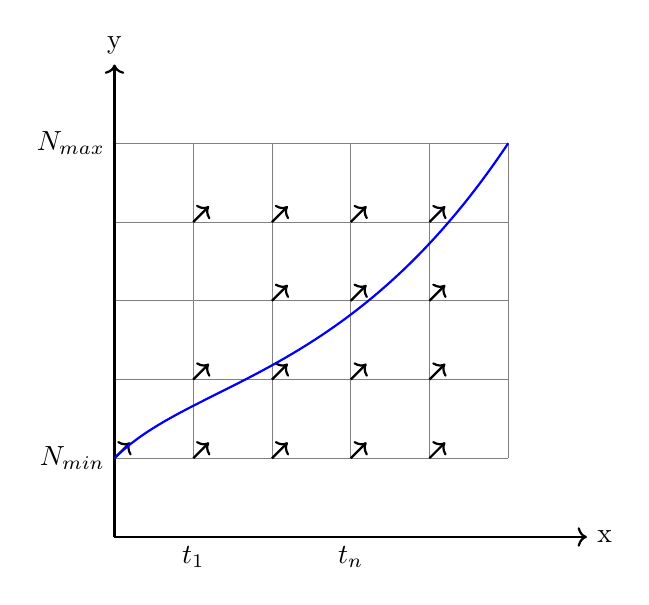
\begin{tikzpicture}
                % Draw the grid
                \draw[step=1cm, gray, very thin] (0,1) grid (5,5);

                % Add axis lines
                \draw[thick,->] (0,0) -- (6,0) node[right] {x};
                \draw[thick,->] (0,0) -- (0,6) node[above] {y};

                \draw[thick,->] (0,1) -- +(0.2, 0.2);
                \draw[thick,->] (1,1) -- +(0.2, 0.2);
                \draw[thick,->] (1,2) -- +(0.2, 0.2);
                \draw[thick,->] (1,4) -- +(0.2, 0.2);
                \draw[thick,->] (2,1) -- +(0.2, 0.2);
                \draw[thick,->] (2,2) -- +(0.2, 0.2);
                \draw[thick,->] (2,3) -- +(0.2, 0.2);
                \draw[thick,->] (2,4) -- +(0.2, 0.2);
                \draw[thick,->] (3,1) -- +(0.2, 0.2);
                \draw[thick,->] (3,2) -- +(0.2, 0.2);
                \draw[thick,->] (3,3) -- +(0.2, 0.2);
                \draw[thick,->] (3,4) -- +(0.2, 0.2);
                \draw[thick,->] (4,1) -- +(0.2, 0.2);
                \draw[thick,->] (4,2) -- +(0.2, 0.2);
                \draw[thick,->] (4,3) -- +(0.2, 0.2);
                \draw[thick,->] (4,4) -- +(0.2, 0.2);
                \node[left] (_) at (0,1){$N_{min}$};
                \node[left] (_) at (0,5){$N_{max}$};
                \draw[thick, blue] (0, 1) .. controls (1,2) and (3,2) .. (5, 5);
                \node[below] (_) at (1, 0){$t_1$};
                \node[below] (_) at (3, 0){$t_n$};
            \end{tikzpicture}  
            \caption{Une courbe sur des champs de vecteurs}
        \end{figure}
\end{enumerate}
Analysons ce que represente le vecteurs tangent:
\begin{itemize}
    \item pour une courbe $y = g(x)$
    \item python et tout autre logiciel procède ainsi
\end{itemize}
\begin{figure}[H]
    \centering
    \incfig{analysons-ce-que-represente-vecteur}
    \caption{Ce que represente vecteur}
    \label{fig:analysons-ce-que-represente-vecteur}
\end{figure}
Le vecteur tangent à la courbe:
\begin{align*}
    \vec{v} = (1, g'(x)) = (1, \frac{dy}{dx}) = (1, \frac{\frac{dy}{dt}}{\frac{dy}{dt}})\\
= \frac{1}{\frac{dy}{dt}}(\frac{dx}{dt}, \frac{dy}{dt}) = \underset{\in \R}{ \frac{1}{\dot{x}(t)} }\underbrace{(\dot{x}(t), \dot{y}(t))}_{\text{vecteur tangent}}
\end{align*}
\[
    \vec{v} = (\dot{x}(t), \dot{y}(t))
\] 
Càd $\vec{v}$ est le vecteur vitesse au points  $M(x(t), y(t))$ a la courbe parametrée  $t \mapsto \begin{cases}
    x(t) = t\\
    y(t) = g(t)
\end{cases}$. On a le résultat.
\begin{prop}
    \begin{align*}
        &\left(\text{y obtient solution de l'EDO } y'(t)=f(t, y(t)) \right) \\
        &\rotatebox{90}{$\iff$}\\ 
        &(\text{vecteur vitesse de la courbe parametrée } t \mapsto (x(t), y(t)) \text{ au point } M(t_0) = (t_0, y(t_0))\\ 
        &\text{ si le vecteur } (1, f(t_0, y(t_0))))  
    \end{align*}
\end{prop}
\begin{prop}
   \begin{align*}
       V: \R^2 &\longrightarrow \R^2 \\
       (t, y) &\longmapsto V((t, y))
   .\end{align*} 
   \[
       \text{(si le champ de vecteur associé à l'EDO } y'(t) = f(t, y(t)) \text{)} \iff V(t, y) = (1, f(t, y))
   \] 
\end{prop}
\subsection{Dessins de champs de vecteurs}
\textbf{\large Principe:}\\
À chaque points $P = (p_x, p_y)$ on trace le vecteur  $\epsilon V(P)$ où  $\epsilon$ est une constance positive choisi pour écrire les vecteurs trop longs.\\
Avec python on écrit \textit{quiver($P_x, P_y, V_x, V_y,$ angles='xy')}
RQ 1: Cette fonction est vectorielle, i.e $P_x, P_y, V_x, V_y,$ sont des numpy array de taille  $n$.
RQ 2: On peut ajouter un paramètre pour controles la longeur des vecteurs:
 \begin{center}
   plt.quiver($P_x, P_y, V_x, V_y$, angles='xy', sacle=$1$) 
\end{center}
Par conséquent, il faut normaliser les vecteurs (i.e le champ de vecteur)
\begin{eg}
   Champ de vecteur du modèle de Verhulst:
   \begin{lstlisting}
       
       def f(t, y):
         return r * y * (1 - y/k)
     \end{lstlisting}
    la grille:

   \begin{lstlisting}
       lt = np.linspace(tmin, tmax, N+1)
       ly = np.linspace(ymin, ymax, M+1)
       T, Y = np.meshgrid(lx, ly)
   \end{lstlisting}
    Construire les vecteurs:

    \begin{lstlisting}
        
       Y = 1 + 0 * T
       V = f(T, Y)
       norm = np.sqrt(U*U + V*V)
        U = U/norm
        V = V/norm
    \end{lstlisting}
    On place les points:
    \begin{lstlisting}
       plt.scatter(T, Y, marker='+', alpha = 0.5)
\end{lstlisting}
    On place les vecteurs
    \begin{lstlisting}
       plt.quiver(T, Y, U, V, angles='xy', scale=N)
\end{lstlisting}
\end{eg}
\subsection{Recherche de solution approchée de modèles sous python}
On cherche une solution approchée de 
\[
\begin{cases}
    y'(t) = f(t, y(t)) \quad t \in ]t_0, t_0 + T[\\
    y(t_0) = y_0
\end{cases}
\] avec python. Pour cela il suffit de dire \textbf{en quels points} on veut cette solution.\\
On se donne:
\begin{itemize}
    \item une liste des instants [$t_0, t_1, \ldots, t_N$]
    \item $t_0, y_0$
    \item Puis, on appelle la fonction \underline{odeint} du module \underline{scipy.integrate} de python.
    \item On obtient une liste [$y_0, y_1, \ldots, y_N$]
\end{itemize}
\begin{eg}
   Cas du modèle du Verhulst 
   \begin{itemize}
       \item EDO:
           \begin{lstlisting}
              def f(t, y):
                return \ldots
           \end{lstlisting}
       \item Instants
           \begin{lstlisting}
              t0, tf = a, b 
              N = 100
              t = np.linspace(t0, tf, N)
           \end{lstlisting}
       \item On appelle odeint
           \begin{lstlisting}
              from scipy.integrate import odeint
              yapp = odeint(f, t, y), rtol=None, atol=None, tfloat=False)
              plt.plot(t, yapp, \ldots)
           \end{lstlisting}
   \end{itemize}
\end{eg}
\section{Modèle de prédateur prose (lotka-voltena (1931))}
$H(t)$: population de sardins\\
$P(t)$: pupulation de reguins
 \[
     \frac{H'(t)}{H(t)} = \text{taux de variation de sardins} = \underbrace{a}_{\text{taux de croissance}} - \underbrace{b P(t)}_{\text{taux de mortalité}}
\] 
\[
    \frac{P'(t)}{P(t)} = \text{taux d'arrivé des requetes} = \underbrace{-c}_{\text{taux de décès}} + \underbrace{d H(t)}_{\text{taux de croissance}}
\] 
D'où le modèle:
\[
\begin{cases}
    H'(t) = H(t)(a - b P(t)) \quad t>0\\
    P'(t) = P(t)(-c + d H(t))\\
    H(0) = H_0, \quad P(0) = P_0
\end{cases}
\] 
Si l'on désigne par $p\ge 0$ la proportion des requêtes en sardines pêchés
\[
\begin{cases}
    H'(t) = H(t)(a - p - b P(t)) \quad t > 0\\
    P'(t) = P(t)(-c - p - d H(t))\\
    H(0) = H_0\\
    P(0) = P_0
\end{cases}
\] 

\chapter{Interpolation polynomiale}
On va essayer de construire des polynôms qui passent par un ensemble (nuages) de points donnés.

Si ces points sont les valeurs d'une fonction, on amerait:
\begin{itemize}
    \item savoir si le polynôme construit est d'autant plus proche de la fonction que le nombre de point est grand. C'est-à-dre, est-ce que nute des "erreurs" tend vers zero lorsque le nombre de points tend vers l'infini.
    \item Si oui, comment quantifier cette convergence? C'est-à-dire, quelle est la vitesse (ordre) de cette convergence.
        \begin{figure}[H]
            \centering
            \incfig{evolution-de-population-en-annee}
            \caption{evolution-de-population-en-annee}
            \label{fig:evolution-de-population-en-annee}
        \end{figure}
\end{itemize}
\begin{enumerate}
    \item Approche 1: approximation linéaire. 
        \begin{itemize}
            \item Polynôme de degré 1
        \end{itemize}
    \item Approche 2: 
        \begin{itemize}
            \item polynôme de degré 2
            \item approximation quadratique
        \end{itemize}
    \item Approche 3: prise en compre d'Historique
\end{enumerate}

\section{Rappels sur les nuts numériques\\
          Vitesse (ordre) de convergence\\
          valeur ajoutée par itérations
      }
\begin{definition}
    Soit $(x_n)_n \subset \R^n$ une suite qui converge vers $x^* \in \R^n$, pour une norme $\| \, \|$ de  $\R^n$
    \begin{itemize}
        \item Si $k_1 = \lim_{x \to \infty} \frac{\|x_{n+1} - x^*\|}{\|x_n - x^*\|}$ existe et $k_1 \in ]-1, 1[ \setminus \{0\}$. On dit que la suite convere \underline{linéairement} vers $x^*$ ou que la convergence est d'ordre  $1$.
        \item Si  $k_1 = 0$, $k_2 = \lim_{n \to \infty} \frac{\|x_{n+1} - x^*\|}{\|x_n - x^*\|^2}$ existe et non nul. On dit que la suite coverge \underline{quadratiquement} vers $x^*$, ou que la convergence est \underline{d'ordre $2$}.  
        \item Si $k_q = \lim_{n \to \infty} \frac{\|x_{n+1} - x^*\|}{\|x_n - x^*\|^q}$ existe et $\neq 0$ la convergence est \underline{ d'ordre $q$ }. La constante $K_q$ est appelée \underline{constante asymptotique d'erreur}.
    \end{itemize}
\end{definition}
\begin{eg}
    \begin{enumerate}
        \item 
   $x_n = (0.2)^n$ 
   \begin{itemize}
       \item On a $\lim_{n \to \infty} x_n = 0$. La convergence vers $x^* = 0$.
       \item  $\lim_{n \to \infty} \frac{|x_{n+1} - x^*|}{|x_n - x^*|} = \lim_{n \to \infty} \frac{(0.2)^{n+1}}{(0.2)^n} = 0.2 \in ]-1, 1[ \setminus \{0\}$
   \end{itemize}
   D'où
   \begin{itemize}
       \item $x_n$ converge à \underline{l'ordre $1$} 
       \item Sa constante asymptotique est \underline{$k_1 = 0.2$}
   \end{itemize}
   \item
       $I_n = (0.2)^{2^n}$. On a  $\lim_{n \to \infty} I_n = 0$\\
       On a:
       \begin{align*}
           I_{n+1} = (0.2)^{2^{n+1}} &= (0.2)^{2^n \cdot 2}\\
                                     &= \left( (0.2)^{2^n} \right)^2\\
                                     &= \left( I_n \right)^2
       \end{align*}
       D'où $\lim_{n \to \infty} \frac{I_{n+1}}{\left( I_n \right)^2} = \lim_{n \to \infty} \frac{\left( I_n \right)^2}{\left( I_n \right)^2} = 1$
       D'où
       \begin{itemize}
           \item convergence \underline{d'ordre $2$}
           \item de constante $k_2 = 1$
       \end{itemize}
\end{enumerate}
\end{eg}
En pratique, on ne dispose pas de $K_q$
 \begin{definition}
    \[
        \substack{x_n \text{ converge vers } x^*\\\text{à l'ordre } q} \implies \exists N \in \N, \exists A,B \in \R \text{ tq } \forall n \ge N, 0 < A \le \frac{\|x_{n+1} - x^*\|}{\|x_n - x^*\|^q} \le B < +\infty
    \] 
    La convergence est au moins d'ordre $q$ si et seulement si on a (deuxieme partie d'équation)
\end{definition}

\subsection{Valeur ajoutée par l'itération}
Il est question de comparer $2$ suites qui ont la même vitesse de convergence.
\begin{remark}
    Si $|x_n - x^*| = 4 \cdot 10^{-8} = 0.\underbrace{0000000}_{7 \text{ chiffres}}4$. On dira que $x_n$ et  $x^*$ ont 7 chiffres exactes apres la virgule.
    \begin{align*}
    &\log_{10} |x_n - x^*| = \log_{10}4 - 8\log_{10}(10)\\
    &\frac{\log|x_n - x^*|}{\log 10} = \frac{\log 4}{\log 10} - 8
    \end{align*}
    i.e $d_n = - \log_{10} |x_n - x^*|$ mesure de nombre de chiffres décimales entre $x_n$ et  $x^*$ qui coincident.
\end{remark}
\begin{remark}
   \[
       \lim_{n \to \infty} \frac{\|x_{n+1} - x^*\|}{\|x_n - x^*\|^q} = K_q \implies K_q \approx \frac{\|x_{n+1} - x^*\|}{\|x_n - x^*\|^q}
   \]  
   D'où $d_{n+1} - q d_n \approx -\log_{10} K_q$, i.e
   \[
   d_{n+1} + \frac{\log_{10} K_q}{1 - q} \approx q(d_n + \frac{\log_{10} K_q}{1 - q})
   \] 
   Donc, le nombre de chiffres significatives est multiplié par $q$.
\end{remark}
\begin{prop}
   Si $x_n$ converge à l'ordre  $1$ vers  $x^*$ de constante asymptotique  $K_1$, alors le nombre d'itérations nécessaires pour gagner un chiffre exacte est la partié enitère de  $-\frac{1}{\log_{10}K_1}$ 
\end{prop}
\begin{preuve}
Soit $m$ le nombre d'itérations pour gegner un chiffre. Comme  $d_{n+1} - d_n = -\log_{10} K_1$, en partant de $d_n$, après  $m$ itérations on aura
 \[
     d_{n+m} - d_{n} = -m \log_{10}K_1
\] 
D'où on aura gagné $1$ chiffre si  $d_{n+m} - d_n = 1$, i.e
\[
1 = -m \log_{10}K_1 \implies m = \left( -\frac{1}{\log_{10}K_1} \right) 
\] 
\end{preuve}

\subsection{Obtenir numériquement la vitesse de convergence}
On cherche $q$ tq:  $\lim_{n \to \infty} \frac{\|x_{n+1} - x^*\|}{\|x_n - x^*\|^q} = K_q \in  \R^*$
\begin{remark}
    \begin{align*}
        &\frac{\|x_{n+1} - x^*\|}{\|x_n - x^*\|^q} \approx K_q
        \implies& \underbrace{ \log \|x_{n+1} - x^*\|  }_{Y} - \underbrace{q \log\|x_n - x^*\|}_{X} = \log K_q
    \end{align*}
    i.e $Y = aX + b$. 
    \par
    Conclusion: pour détérminer q:
     \begin{itemize}
        \item Traiter la courbe $\log\|x_n - x^*\| \mapsto \log\|x_{n+1} - x^*\|$
        \item Détérminer $q$ comme la parte de la droite passant par le maximum de points.
    \end{itemize}
\end{remark}
\begin{align*}
    &x_n = x_0, x_1, \ldots, x_N\\
    &x_n - x^* = x_0 - x^*, x_1 - x^*, \ldots, x_N - x^*\\
    &x_{n+1} - x^* = x_1 - x^*, x_2 - x^*, \ldots, x_{N+1} - x^*
\end{align*}
En python:

\begin{lstlisting}
xn = np.array([x0, ..., xN])
e = np.log(np.abs(xn - x^*))
ex = e[0:-1] #de premier a avant dernier
ey = e[1:] #de deuxieme au dernier
plt.scatter(ex, ey, label="miage")
a,b = np.polyfit(ex, ey, 1)
plt.plot(ex, b + a * ex, label=f"$x \mapsto {b:32f} + {a:32f}x$")
\end{lstlisting}

\section{Interpolation: définition-motivation-exemples}
\subsection{Définition}
\begin{definition}
    Soient $(x_i, y_i)_{i = \{1, \ldots, N\}}$ un nuage de points(exemple un ensemble discret de point du graphe d'une fonction). Interpoler ce nuage de points correspond à chercher un polynôme de degré $N-1$, qui passe par chacun de ces points.
\end{definition}
\begin{figure}[H]
    \centering
    \incfig{definition-example}
    \caption{L'exemple visuel de la définition}
    \label{fig:definition-example}
\end{figure}
Questions:
\begin{enumerate}
    \item Comment le construire?
    \item $P_{N-1} \in \R_{N-1}[X]$
    \item $P_{N-1}(x_i) = y_i$
\end{enumerate}

\subsection{Motivations}
\begin{itemize}
    \item La solution d'un problème est fournie par une formule représentative: Noyau de la chaleur (i.e convolution) est un cherche la solution en un nombre de points.
    \begin{itemize}
        \item On approche alors la fonction par un polynôme: i.e chercher le polynôme de degré "bas" proche de la fonction
    \end{itemize}
    \item La solution d'un problème n'est connue qu'à table des valeurs en un nombre fini de points et on souhaite l'évaluer partout.
        \begin{itemize}
            \item l'intérpolation
        \end{itemize}
    \item On peut utiliser l'intérpolation dans 
        \begin{itemize}
            \item l'intégration numérique
            \item la résolution numérique des EDO
            \item la visualisation scientifique
        \end{itemize}
\end{itemize}

\begin{definition}
    Un tel polynôme est appelé \textbf{polynôme intérpolateur de lagrange} de degré $N-1$ de ces points.
\end{definition}
\subsection{exemples d'intérpolation}
\begin{theorem}
    Polynôme intérpolateur de degré 1.
    \par
    Soient $(x_1, y_1), \, (x_2, y_2)$ 2 points distincts de $\R^2$
    \begin{itemize}
        \item Il existe une unique droite passant par les 2 points.
            \[
                (x, y) \in \mathcal{D} \iff (x-x_1)(y_2 - y_1) - (y - y_1)(x_2 - x_1) = 0
            \] 
        \item Si de plus, $x_1 \neq  x_2$, il existe un unique polynôme de degré $1$ (i.e $P_1 \in \R_1[X]$) tq:
            \[
                (x, y) \in \mathcal{D} \iff y = P(x) \text{ avec } P_1 = \frac{(x - x_1)y_1 - (x - x_2)y_2}{x_2 - x_1}
            \] 
    \end{itemize}
\end{theorem}
\begin{preuve}
    \begin{itemize}
        \item 
    \begin{align*}
        M \begin{pmatrix} x \\ y \end{pmatrix} \in \mathcal{D} &\iff \vec{MM_1} / \vec{M_1M_2}\\
                                                               &\iff det(\vec{MM_1}, \vec{M_1M_2}) = 0\\
                                                               &\iff \begin{vmatrix} x - x_1 & x_2 - x_1 \\ y - y_1 & y_2 - y_1 \end{vmatrix} = 0\\
                                                               &\iff (x - x_1)(y_2 - y_1) - (y - y_1)(x_2 - x_1) = 0
    \end{align*}
\item Si $x_1 \neq x_2$
    \begin{align*}
        M \in \mathcal{D} &\iff y - y_1 = \frac{(x - x_1)(y_2 - y_1)}{x_2 - x_1}\\
                          &\iff y = P_1(X)
    \end{align*}
\end{itemize}
\end{preuve}
\begin{remark}
    On a l'écriture équivalente de $P_1$:
   \begin{itemize}
       \item 
           \[
               P_1 \frac{x_0y_1 - x_1y_2}{x_2 - x_1} + X \frac{y_2 - y_1}{x_2 - x_1} \equiv a_0 + a_1X
           \] 
           C'est l'écriture dans la base $(1, X)$ de  $\R_1[X]$
       \item 
           \[
               P_1 = \underbrace{ \frac{x - x_2}{x_1 - x_2} }_{l_1}y_1 + \underbrace{ \frac{x - x_1}{x_2 - x_1} }_{l_2}y_2
           \] 
           C'est l'écriture dans la base $(l_1, l_2)$ de $\R_1[X]$
           \par
           RQ:
           \[
           l_1(x_1) = 1 \quad l_1(x_2) = 0 \quad l_2(x_1) = 0 \quad l_2(x_2) = 1
           \] 
           (base de lagrange)
        \item 
            \[
            P_1 = y_1 + \frac{y_2 - y_1}{x_2 - x_1}(x - x_1)
            \] 
            C'est l'écriture dans la base $(1, x - x_1)$ de $\R_1[X]$ (base de newton)
   \end{itemize} 
\end{remark}
\begin{eg}
   Méthode de calcul employle 
   \par
   Chercher le polynôme interpolateur de lagrange aux points $(x_1, y_1), (x_2, y_2), (x_3, y_3)$
   \begin{itemize}
       \item \underline{Méthode 1}: $x_1 \neq x_2 \neq x_3$ \par
           $P_2$ est un polynôme de degré 2
           \[
           P_2 = a_0 + a_1x + a_2x^2
           \] 
           \begin{lemma}
              \[
              P_2(x_1) = y_1, \quad P_2(x_2) = y_2 \qquad \text{i.e } a_0 + a_1x_1 + a_2x_1^2 = y_1
              \]  
           \end{lemma}
           \[
               \underbrace{
                   \begin{bmatrix} 
                       1 & x_1 & x_1^2\\
                       1 & x_2 & x_2^2\\
                       1 & x_3 & x_3^2
                   \end{bmatrix} 
               }_{M}\underbrace{\begin{bmatrix} a_0 \\ a_1 \\ a_2 \end{bmatrix} }_{} = \underbrace{\begin{bmatrix} y_1 \\ y_2 \\ y_3 \end{bmatrix} }_{} \implies \begin{bmatrix} a_0 \\ a_1 \\ a_2 \end{bmatrix} = \underbrace{M^{-1}}_{???}\begin{bmatrix} y_1 \\ y_2 \\ y_3 \end{bmatrix} 
           \] 
           \begin{remark}
              Par 2 points 
              \[
                  M = \begin{bmatrix} 1 & x_1 \\ 1 & x_2 \end{bmatrix} \text{ et } M^{-1} = \frac{1}{x_2 - x_1}\begin{bmatrix} x_2 & -x_1\\ -1 & 1 \end{bmatrix} 
              \] 
           \end{remark}
        \item \underline{Méthode 2}:\par
            \[
            P_2 = a_0 + a_1(x - x_1) + a_2(x - x_1)(x - x_2)
            \] 
            \begin{align*}
                \underset{i = 1,2,3}{P_2(x_i) = y_i} \implies &\begin{cases}
                    a_0 &=y_1\\
                    a_0 + a_1(x_2 - x_1) &= y_2\\
                    a_0 + a_1(x_3 - x_1) + a_2(x_3 - x_1)(x_3 - x_2) &= y_3
                \end{cases}\\
                                                        \implies &\begin{cases}
                                                                  a_0 &= y_1\\
                                                                  a_1 &= \frac{y_2 - y_1}{x_2 - x_1}\\
                                                                  a_2 &= \frac{y_3 - y_1 - \frac{y_2 - y_1}{x_2 - x_1}(x_3 - x_1)}{(x_3 - x_1)(x_3 - x_2)}
                                                              \end{cases}
            \end{align*}
            \begin{remark}
               On a:
               \[
               a_2 = \frac{\frac{y_2 - y_1}{x_2 - x_1} - \frac{y_3 - y_2}{x_3 - x_2}}{x_3 - x_1}
               \] 
               càd 
               \[
               P_3 = y_1 + \frac{y_2 - y_1}{x_2 - x_1}(x - x_1) + \frac{\frac{y_2 - y_1}{x_2 - x_1} - \frac{y_3 - y_2}{x_3 - x_2}}{x_3 - x_2}(x-x_1)(x-x_2)
               \] 
               \begin{center}
                   \begin{tabular}{| c | c | c | c |}
                       \hline
                   $x_1$ & $y_1 =: a_3$ &  &  \\
                       \hline
                   $x_2$ & $y_2$ & $\frac{y_2 - y_1}{x_2 - x_1} =: a_1$ & \\
                   \hline
                   $x_3$ & $y_3$ & $\frac{y_3 - y_2}{x_3 - x_2}$ & $\frac{\frac{y_2 - y_1}{x_2 - x_1} - \frac{y_3 - y_2}{x_3 - x_2}}{x_3 - x_1} =: a_2$\\
                   \hline
                   \end{tabular}
               \end{center}
            \end{remark}
        \item \underline{Méthode 3}:
            \par
            \[
            P_3 = \frac{(x - x_2)(x - x_3)}{(x_1 - x_2)(x_1 - x_3)}y_1 + \frac{(x - x_1)(x - x_3)}{(x_2 - x_1)(x_2 - x_3)}y_2 + \frac{(x - x_1)(x - x_2)}{(x_3 - x_1)(x_3 - x_2)}y_3 = \sum_{i=1}^{3} \underbrace{\left( \prod_{j=1}^{3} \frac{x - x_j}{x_i - x_j}  \right)}_{l_i(x)} y_i
            \] 
            \begin{remark}
               $(x_1, y_1), (x_2, y_2)$ 
               \[
               y = \frac{x - x_2}{x_1 - x_2}y_1 + \frac{x - x_1}{x_2 - x_1}y_2
               \] 
            \end{remark}
   \end{itemize}
\end{eg}
\section{Polynôme interpolateur de lagrange}
\subsection{Définition et propriétés}
\begin{theorem}
    (existence et utilité) \par
    Soit $x_1, \ldots, x_n$ des réels 2 à 2 distincts et $y_1, \ldots, y_n$ des rééls quelconques: Il existe \underline{un unique} polynôme $P \in \R_{n-1}[X]$ (i.e de degré $n-1$) tel que $p(x_i) = y_i, \, i = 1, \ldots, n$
    \par
    On dit que $P$ est le polynôme interpolateur de lagrange aux points  $(x_1, y_1), \, \ldots, \, (x_n, y_n)$
\end{theorem}
\begin{preuve}
   Soit \begin{align*}
       \Phi: \R_{n-1}[X] &\longrightarrow \R^{n-1} \\
       P &\longmapsto \Phi(P) = (P(x_1), \ldots, P(x_n))
   .\end{align*} 
   on a:
   \begin{itemize}
       \item $\Phi$ linéaire
       \item  $\Phi$ injective
   \end{itemize}
   En effet, $\Phi(P) = 0 \iff P(x_i) = 0 \iff P \equiv 0$ car $deg(P) \le n-1$.
   D'où $\Phi$ isomorphisme d'espace vectoriel et la surjection assure le résultat.
\end{preuve}
\begin{definition}
    Si $f$ est continue sur  $[a, b] \to \R$, $x_1, \ldots, x_n \in [a, b]$ 2 à 2 distincts, alors, l'unique $P \in \R_{n-1}[X]$ tq $P(x_i) = f(x_i) \, i = 1, \ldots, n$ est appelé \underline{polynôme d'interpolation de lagrange} de $f$ aux points  $x_1, \ldots, x_n$
\end{definition}
\subsection{Estiomation d'erreur}
\begin{theorem}
    l'erreur  \par
    Soient
    \begin{itemize}
        \item $a < b$  $f: [a, b] \to \R$ continue
        \item $x_1, \ldots, x_n$ 2 à 2 distincts de $[a, b]$
        \item  $P$ polyôme d'interpolation de lagrange de  $f$ aux points  $x_i$
    \end{itemize}
    Si $f$ est $n$ fois dérivable sur  $]a, b[$, alors, pour tout  $a \in [a, b]$, il existe  $t \in ]a, b[$ tq 
     \[
         f(x) - P(x) = \omega_n(x)\frac{f^{(n)}(t)}{n!}
    \] 
    où $\omega_n(x) = (x - x_1)\ldots(x - x_n)$
\end{theorem}
\begin{corollary}
    Si $f^{(n)}$ est bornée par  $M$ sur  $]a, b[$, alors  $\forall x \in [a, b]$ 
    \[
    |f(x) - P(x)| \le \frac{M}{n!}|\omega_n(x)| \le \frac{M}{n!}(b - a)^n
    \] 
\end{corollary}
\begin{preuve}
    à faire
\end{preuve}

\subsection{Implémentation avec python}
\begin{lstlisting}
   from scipy.interpolite import lagrange
   x = np.array([x_1, x_2, x_3])
   y = np.array([y_1, y_2, y_3])
   p = lagrange(x, y)
   print(p) # affiche le polynome
   print(p(3)) # collable
\end{lstlisting}

\section{Construction des polynôme d'intérpolation de lagrange}
$x_0, \ldots, x_{n-1}$ 2 à 2 distincts
\subsection{Interpolation dans la base canonique (Vandermonde)}
\subsubsection{Construction}
\[
P = \sum_{i=1}^{n-1} a_ix^i
\] 
\[
P(x_i) = y_i, \, i = 0, \ldots, n-1
\] 
\[
    \underbrace{
        \begin{bmatrix} 
            1 & x_0 & \ldots & x_0^{n-1}\\
            1 & x_1 & \ldots & x_1^{n-1}\\
            \ldots & \ldots & \ldots & \ldots\\
            1 & x_{n-1} & \ldots & x_{n-1}^{n-1}
        \end{bmatrix} 
    }_{V(x_0, \ldots, x_{n-1})} \underbrace{\begin{bmatrix} a_0 \\ \ldots \\ a_{n-1} \end{bmatrix} }_{a} 
    =
    \underbrace{\begin{bmatrix} y_1 \\ \ldots \\ y_{n-1} \end{bmatrix} }_{b}
\] 
Matrice de Vandermonde
\begin{itemize}
    \item elle pleine
    \item malconditionnée
\end{itemize}
\begin{lstlisting}
def VDM_Mat(x):
    x_n = np.reshape(x, (x.size, 1))
    return x_n ** np.arange(x.size)
\end{lstlisting}
\begin{lstlisting}
def VDM_Poly(x, y):
    M = VDM_Mat(x)
    a = np.linalg.solve(M, y)
    return a
\end{lstlisting}
\subsubsection{Evaluation efficace de $P$ algorithme de Horner}
\begin{prop}
   Si $X$ est un réel et  $Q$ est le polynôme défini par 
   \[
       Q(X) = a_0X^n + a_1X^{n-1} + \ldots + a_{n-1}X + a_n
   \] 
   alors la suite
   \[
   \begin{cases}
       q_0 = a_0\\
       q_k = q_{k-1}x + a_k, \, k=1,\ldots,n
   \end{cases}
   \] 
   vérfiie $q_n = Q(x)$
\end{prop}
\begin{preuve}
    (laissé exo)
    \[
    Q(X) = X^2 + 2X + 1 \equiv (X+2)X + 1
    \] 
\end{preuve}
\begin{lstlisting}
def Horner(P, xx): 
   y = 0
   for a in P:
        y = y * xx + a
   return y
\end{lstlisting}
\begin{lstlisting}
def IntuP_VDM(x, y, xx):
    a = VDM_Poly(x, y)
    yy = Horner(a[::-1], xx)
    return yy
\end{lstlisting}
\subsection{Interpolation dans la base duale: Formule de lagrange et points barycentrique}
\subsubsection{Construction}
Idée prendre pour base de $\R_{n-1}[X]$ l'image réciproque de la base canonique de $\R^{n-1}$ pour $\Phi$ 
\[
L_i(x_j) = \begin{cases}
    1 \text{ si } i \neq j\\
    0 \text{ sinon}
\end{cases}
\] 
\[
    L_i(x) = \frac{\prod_{j\neq i \, j = 0}^{n-1}(x - x_j) }{\prod_{j = 0 \, j \neq i}^{n-1} (x_i - x_j) } = \prod_{j = 1 \, j \neq i}^{n-1} \frac{x - x_j}{x_i - x_j} 
\] 
\[
P(X) = \sum_{i=0}^{n-1} y_iL_i(X)
\] 

\begin{theorem}
    \begin{align*}
        &f: [a, b] \to \R \\
        &x_1, \ldots, x_n \\
        &P
    \end{align*}
    Si $f$  $n$ fois dérivable,  
    \[
        \forall x \in [a, b], \, \exists t \in ]a, b[, f(x) - P(x) = \omega_n(x)\frac{f^{(n)}(t)}{n!}
    \] 
\end{theorem}
\begin{preuve} du théorème (erreur)
    \par
    Soit x fixé des $[a, b] \setminus \{x_1, \ldots, x_n\}$
    \par
    On pose 
    \[
    F(t) = f(t) - P(t) - \frac{f(x) - P(x)}{\omega_n(t)}\omega_n(t)
    \] 
    $F$ est  $n$ fois dérivable et  $P$ annule aux  $n+1$ points  $x_1, \ldots, x_n, x$. D'apres le théorème Rolle (généralisé) 
    \[
        \exists t \in ]a, b[ \text{ tq } f^{(n)}(t) = 0
    \] 
    Or
    \[
        \underbrace{F^{(n)}(t)}_{= 0 \text{ par hyp}} = f^{(n)}(t) - \underbrace{P^{(n)}(t)}_{= 0 \text{ car } deg(P) < n} - \frac{f(x) - P(x)}{\omega_n(x)}n!
    \] 
    D'où
    \[
        f(x) - P(x) = \omega_N(x) \frac{f^{(n)}(t)}{n!}
    \] 
    Par ailleurs, si $x \in \{x_1, \ldots, x_n\}, \, f(x) - P(x) = 0$
    \[
    \omega_n(x) = (x - x_1)\ldots(x - x_n)
    \] 
\end{preuve}
\begin{preuve} corollaire
   \[
       |f(x) - P(x)| = |\omega_n(x)| \frac{|f^{(n)}(t)|}{n!}
   \]  
   comme $x, x_i \in [a, b]$, on a  $|x - x_i| \le b - a$ et $|f^{(n)}(t)| \le M$, on a:
   \[
   |f(x) - P(x) \le \frac{M}{n!}(b - a)^n
   \] 
\end{preuve}

\subsubsection{Evaluation efficace: formule barycentrique}
\begin{prop}
   On a 
   \begin{align*}
       P(x) &= \sum_{i=1}^{n} y_i \frac{\omega_n(x)}{(x - x_i)\omega_n'(x_i)}\\
            &= \frac{\sum_{i=1}^{n} \frac{1}{(x - x_i)\omega_n'(x_i)}y_i}{\sum_{i=1}^{n} \frac{1}{(x - x_i)\omega_n'(x_i)}}
   \end{align*}
\end{prop}
\begin{preuve}
   Comme 
   \[
   \omega_n(x) = \prod_{i=1}^{n} (x - x_i) \implies \omega_n'(x) = \sum_{i=1}^{n} \prod_{j=1 \quad j \neq 1}^{n} (x - x_j)  
   \] 
   D'où
   \[
   \omega_n'(x_i) = \prod_{j=1 \quad j \neq i}^{n} (x_i - x_j) \quad i = 1, \ldots, n
   \] 
   D'où 
   \[
   L_i(x) = \frac{\omega_n(x)}{x - x_i}\frac{1}{\omega_n'(x_i)}
   \] 
   Et 
   \begin{align*}
       \sum_{i=1}^{n} y_iL_i(x) &= \sum_{i=1}^{n} \frac{y_i}{(x - x_i)\omega_n'(x)}\omega_n(x)\\
                                &= \omega_n(x) \sum_{i=1}^{n} \frac{y_i}{(x - x_i)\omega_n'(x_i)}
   \end{align*}
   Or pour $P \equiv 1$ on a  $y_i = 1, i = 1, \ldots, n$, on a
   \[
   1 = \omega_n(x) \sum_{i=1}^{n} \frac{1}{(x - x_i)\omega_n'(x)}
   \] 
   D'où
   \[
       \omega_n(x) = \left(   \sum_{i=1}^{n} \frac{1}{(x - x_i)\omega_n'(x)}\right)^{-1}
   \] 
   Enfin,
   \[
   P(x) = \frac{\sum_{i=1}^{n} \frac{y_i}{(x - x_i)\omega_n'(x)}}{\sum_{i=1}^{n} \frac{1}{(x - x_i)\omega_n'(x)}}
   \] 
\end{preuve}
\begin{remark}
   \begin{enumerate}
       \item Attention: si $x = x_i, \, i = 1, \ldots, n$
       \item Exercice: calculer la complexité de cette formule et comparer à la première.
       \item Ajouter un nouveau point d'interpolation ablige à refaire tous les calculs.
   \end{enumerate} 
\end{remark}

\subsection{Méthode des différences divisées}
\subsubsection{Préliminaires: Interpolation de Neville}
\begin{lemma}
   Considérons $n$ points 2 à 2 distincts $x_1, \ldots, x_n$ et $n$ réels  $y_1, \ldots, y_n$. Pour $1 \le k \le l \le n$, posons $P_{x_k, \ldots, x_l}$ le polynôme d'interpolation aux points 
   \[
       (x_k, y_k) \ldots (x_l, y_l)
   \] 
   Nous avons
   \[
       P_{x_k, \ldots, x_l}(x) = \frac{(x - x_l)P_{x_l \ldots x_{l - 1}}(x) - (x - x_k)P_{x_{k+1}\ldots x_l}(x)}{x_k - x_l}
   \] 
   Schématiquement
   \[
       P(x) = \underbrace{x_k, \overbrace{x_{k+1}, \ldots, x_{l-1}}_{P_1}, x_l}^{P_2}
   \] 
   \[
   \frac{x - x_l}{x_k - x_l}P_1 + \frac{x - x_k}{x_l - x_k}P_2
   \] 
\end{lemma}

\subsubsection{Construction de l'intérpolation de Newton}
\begin{definition} (Polynôme de Newton)
    Soit $n \ge 1$ entier, $x_1, \ldots, x_n$ $n$ rééls 2 à 2 distincts. Les polynômes de Newton  $\omega_0, \ldots, \omega_n$ associés à ces points sont définis par
    \[
    \begin{cases}
        \omega_0 = 1\\
        \omega_j = (x - x_1) \ldots (x - x_j), \quad (1 \le j \le n)
    \end{cases}
    \] 
\end{definition}
\begin{remark}
    $\{\omega_j\}_{j = 1, \ldots, k}$ est une base de $\R_k[x]$    
    \begin{itemize}
        \item Ainsi le polynôme d'intérpolation de Lagrange associé aux points $(x_1, y_1) \ldots (x_n, y_n)$ s'écrit
            \[
            P = \sum_{k=0}^{n-1} \alpha_k\omega_k
            \] 
            où $\alpha_k$ sont solutions de 
             \[
            y_i = \sum_{k=0}^{n-1} \alpha_k\omega_k(x_i), \quad i = 1, \ldots, n
            \] 
    \end{itemize}
\end{remark}
On parle de développement de Newton du polyôme de Lagrange

\begin{definition}
    On appelle differences divisées d'ordre $j-1$ ($1 \le j \le n$) associées aux points $(x_1, y_1), \ldots, (x_i, y_i)$ les nombres $d_{i, j}$ ($i = j$ à $n$) définis par
    \begin{itemize}
        \item $d_{i, 1} = y_i \quad i = 1, \ldots, n$
        \item $d_{i, j} = \frac{d_{i, j-1} - d_{i-1,j-1}}{x_i - x_{i - j + 1}}$ \quad $j = 2$ à $n$, $i = j$ à $n$
    \end{itemize}
    Lorsque $y_i = f(x_i) \quad i = 1, \ldots, n$, $d_{i, j}$  est généralement noté $f[x_{j-i+1}, \ldots, x_{j-1}, x_j]$ et est appelé difference divisé d'ordre $j-1$ aux  $i$ points  $x_{j - i + 1}, \ldots, x_j$
\end{definition}
Python:
\begin{lstlisting}
def MatriceDifferencesDivisee(x, y):
    n = len(y)
    d = np.zeros((n, n))
    d[:, 0] = 1.0 * y
    for j in range(1, n):
        d[j:n, j] = (d[j:n, j-1] - d[j-1:n, j-1]) / (x[j:n] - x[0:n-j])
    return d
\end{lstlisting}
\begin{remark}
   \begin{itemize}
       \item Le "stencil" (squelette) est
           \begin{center}
              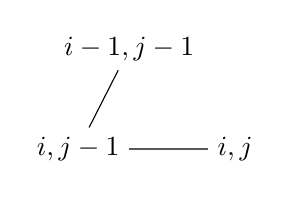
\begin{tikzpicture}
                  \node[above] (a) at (0, 1){$i-1, j-1$};
                  \node[left] (b) at (0, 0){$i, j-1$};
                  \node[right] (c) at (1, 0){$i, j$};
                  \draw (a) -- (b) -- (c);
              \end{tikzpicture} 
           \end{center}
        \item La hauteur de stencil est $j$
        \item Le support du stencil est  $[x_{i-j}, \ldots, x_{i}]$
   \end{itemize} 
\end{remark}
\begin{prop}
    On a $d_{j,j} = \alpha_{j-1}$  pour $j \in [1, \ldots, n]$, càd:
    \[
    P = \sum_{j=1}^{n} d_{j,j}\omega_{j-1}
    \] 
    Ainsi, pour calculer $P$ il suffit de connaître  $d_{j, j} \quad j = 1, \ldots, n$
\end{prop}

\subsubsection{Calcul efficace du polynôme}
\begin{prop}
   Soit donné $x_0, \ldots, x_n$ dés rééls 2 à 2 distincts. Soit $Q$ le polyôme défini par 
   \[
   Q(x) = a_0 + \sum_{i=1}^{n} a_i \prod_{j=1}^{i-1} (x - x_j) \equiv \sum_{i=0}^{n} a_i\omega_i(x) 
   \] 
   La suite des polynômes $Q_0, \ldots, Q_n$ définies par
   \[
   \begin{cases}
       Q_n = a_n\\
       Q_k = a_k + (x - x_k)Q_k \quad k = n-1, \ldots, 0
   \end{cases}
   \] 
   vérifie $Q_0 = Q$
\end{prop}
\begin{lstlisting}
def HornerNewton(d, x, xx):
    n = len(d)
    yy = 0 * xx + d[n-1]
    for i in range(n-2, -1, -1):
        yy = d[i] + (xx - x[i]) * yy
    return yy
\end{lstlisting}
\begin{lstlisting}
def DifferencesDivisees(x, y):
    d = MatriceDifferencesDivisee(x, y)
    a = np.diag(d)
    return a
\end{lstlisting}

\section{Comportement asymptotique "lorsque $N \to \infty$"}
\subsection{Observation}
On n'a pas toujours une convergence uniforme de l'interpolation
\begin{eg}
    $f(x) = \sqrt{x}$ avec $[a, b] = [0, 1]$,  $x_1, \ldots, x_n$ équirépartis sur $[a, b]$ 
    \[
        \underset{a \le t \le b}{max}|f(t) - P(t)| \xrightarrow[n \to \infty]{} +\infty
    \] 
    ce phénomène est appelé \underline{phénoème de Runge}.
\end{eg}

Il en reste une solution: 
\begin{itemize}
    \item si $f$ est lipschitziènne sur  $[a, b]$ ou Hölderienne 
         \[
             \exists a \in ]0, 1[, |f(x) - f(y)| \le C|x - y|
        \] 
    \item Si $x_1, \ldots, x_n$ sont les racines du n-ème polynôme de Tchebychev.
        \[
            |f(x) - P(x)| \le \frac{|f^{(n)}(x)}{n!}\prod_{i=1}^{n} (x - x_i)  
        \] 
\end{itemize}

\subsection{Polynôme de Tchebychev}
\begin{definition}
    Les polynômes de Tchebychev sont définis par la recurrence:
    \[
    \begin{cases}
        T_0 = 1\\
        T_1 = x\\
        T_n = 2xT_{n-1} - T_{n-2} \quad n\ge 2
    \end{cases}
    \] 
\end{definition}
\begin{prop}
   Le n-ième polynôme de Tchebychev vérifie:
   \begin{enumerate}
       \item $T_n$ est de degré exactement  $n$ et son coefficient de plus haut degré est  $2^{n-1}$,  $n \ge 1$
       \item $T_n$ a  $n$ racines distinctes simples
            \[
                T_n(x) = 0 \iff x \in \{x_1, \ldots, x_n\}, x_j = \cos( \frac{2j - 1}{2n} \pi)  \quad (1 \le j \le  n)
           \] 
       \item $|T_n(x)| \le 1, \quad \forall x \in [-1, 1], |T_n(x) = 1 \iff x \in \{x_0, \ldots, x_n\} x_k = \cos(k\frac{\pi}{n})$
           \[
               |T_n(x)| = 1 \text{ si } x \in \{x_k\} \quad x_k = \cos(k\frac{\pi}{n}) \quad (0 \le k \le n)
           \] 
   \end{enumerate}
\end{prop}

\begin{preuve}
    \begin{enumerate}
        \item 
   Par récurrence:
   \par
   Soit $(P_n)$ la propriété "$T_n$ est de degré  $n$ et son coef. de plus haut degré est  $2^{n-1}$", $n\ge 1$. $P_0$ et $P_1$ vraies ($k \le n$). \par
   Supposons $P_k$ vrai et montrons que  $P_{n+1}$ vrai. \par
   En effet, nous avons $T_{n+1} = 2xT_n - T_{n-1}$, on en déduit que $P_{n+1}$ est vraie.\par
   Maintenant,
   \[
       \forall x \in [-1, 1], T_n(x) = \cos(n \cdot \arccos(x))
   \] 
   En effet, pour $\begin{cases}
       n = 0, T_0(x) = 1 = \cos(0)\\
       n = 1, T_n(x) = \cos(\arccos(x))
   \end{cases}$ et  $n > 1$
    \begin{align*}
       \cos((n+1)\arccos(x)) = \cos(n\arccos(x))\cos(\arccos(x)) - \sin(n\arccos(x))\sin(\arccos(x))\\
       \cos((n-1)\arccos(x)) =  \cos(n\arccos(x))\cos(\arccos(x)) + \sin(n\arccos(x))\sin(\arccos(x))\\
   \end{align*}
   On a:
   \[
   \cos((n+1)\arccos(x)) = 2x\cos(n\arccos(x)) - \cos((n-1)\arccos(x))
   \] 
   D'où $x \mapsto \cos(n\arccos(x))$ vérifie la même récurrence sur $[-1, 1]$ que  $T_n$. Par conséquent les 2 coïncident sur  $[-1, 1]$. On en déduit $\forall x \in [-1, 1]$
   \item
   \begin{align*}
       T_n(x) = 0 &\iff \cos(n\arccos(x)) = 0\\
                  &\iff n\arccos(x) = \frac{\pi}{2} \text{ mod } \pi \\
                  &\iff \arccos(x) = \frac{\pi}{2n} \text{ mod } \frac{\pi}{n}
                  &\iff x = \cos(\frac{\pi}{2n} + k\frac{\pi}{n}) \quad 0 \le k \le n-1
   \end{align*}
\item $|\cos(x)| \le 1$ D'où $|T_n(x)| \le 1, \forall x \in [-1, 1]$
    \begin{align*}
        |T_n(x)| = 1 \iff n&\arccos(x) = 0 \text{ mod } \pi\\
                           &\arccos(x) = 0 \text{ mod } \frac{\pi}{n}
    \end{align*}
    \[
        \in x \in \{\cos(k\frac{\pi}{n}), k \in [0, n] \}
    \] 
\end{enumerate}
\end{preuve}

\begin{prop}
   Si $Q_n$ est un polyôme de degré  $n$ de même coeff. de plus haut degré que  $T_n$, alors:
   \[
       \underset{x \in [-1, 1]}{max} |Q_n(x)| \ge \underset{x \in [-1, 1]}{max} |T_n(x)| = 1
   \] 
\end{prop}

\begin{corollary}
    Si $\xi_1, \ldots, \xi_n$  sont $n$ points  $2$ à  $2$ distincts de  $[-1, 1]$, on a:
     \[
         \underset{x \in [-1, 1]}{max} \left| \prod_{j=1}^{n} (x - \xi_{j})  \right| \ge \underset{x \in [-1, 1]}{max} \left| \prod_{j=1}^{n} (x - x_j)  \right| = \underset{x \in [-1, 1]}{max} \frac{1}{2^{n-1}} |T_n(x)| = \frac{1}{2^{n-1}}
    \] 
    où $x_j$ sont les racines de  $T_n$
\end{corollary}

\subsection{Application}
Soit $\xi_1, \ldots, \xi_n$, 2 à 2 distincts, $P$ le polynôme de lagrange de  $f$ (suffisament régulière), alors:
 \begin{align*}
     |f(x) - P(x)| &\le \frac{\|f^{(n)}\|_{\infty}}{n!}|\omega_n(x)|\\
                   &\le \frac{\|f^{(n)}\|_{\infty}}{n!}\|\omega_n(x)\|_{\infty}
\end{align*}
où $\omega_i = \prod_{j=1}^{n} (x - \xi_j) $ et $\| . \|_{\infty}$ et loi norme inf sur $[-1, 1]$. Ainsi, le choix de $\xi_i$ qui possede la plus petite valeur de  $\| \omega_n\|_{\infty}$ est celui des racines du n-ìeme polynôme de Tchebychev.

\begin{remark}
    On se ramène à un intervalle quelconque $[a, b]$ par 
    \[
    x_j = \frac{a + b}{2} + \frac{b - a}{2}\cos(\frac{2j - 1}{2n}\pi) \quad (1 \le j \le n)
    \] 
    sont les racines des polynômes de Tchebychev sur $[a, b]$
\end{remark}


\chapter{Intégration numérique}
\underline{But:} On souhaite calculer au mieux
\[
I(f) = \int_{{a}}^{{b}} {f(x)} \: d{x} {} 
\] 
où $f: [a, b] \to \R$ donné
\par
\underline{Contraintes}
\begin{itemize}
    \item $f$ n'a pas de primitive connue (ou évidente)
    \item  $f$ n'est connue ou ne peut être évaluée qu'en un certain nombre fini de points 
         \[
             (x_i, 0\le i \le n \text{ sur } [a, b])
        \] 
\end{itemize}

\begin{figure}[H]
    \centering
    \incfig{integration-exemple}
    \caption{Exemple d'une intégration}
    \label{fig:integration-exemple}
\end{figure}

\[
I(f) = \int_{{a}}^{{b}} {f(x)} \: d{x} {}
\] 
\[
    S(f, \sum_{N} = \sum_{i=0}^{N} f(\xi_i)\underbrace{(x_{i+1} - x_{i})}_{\omega_i}
\] 
somme de Rieman associée à $\sum_{N}$. Théorème: $\lim_{N \to \infty} S(f, \sum_{N}) = \int_{{a}}^{{b}} {f(x)} \: d{x} {}$

\section{Formule de quadrature}
\begin{definition}
    Étant donnée $N$ points  $x_1, \ldots, x_N$ de l'intervalle $[a, b]$  et $N$ poids  $\omega_1, \ldots, \omega_N \in \R$ associées à chaque points.
    \par
    On appelle \underline{formule de quadrature} associé aux $(x_i),(\omega_i)$ l'application linéaire sur  $\mathcal{C}^0([a, b])$
     \[
         \tilde{I}(f) = \sum_{i=1}^{N} \omega_i f(x_i)
    \] 
    On dit que la formule de quadrature est \underline{d'ordre} $p$ si elle est \underline{exacte} pour les polynôme de degré  $p_1$. i.e
     \[
         \tilde{I}(Q) = \int_{{a}}^{{b}} {Q} \: d{x} {} \forall Q \in \R_{p-1}[X]
    \] 
    et s'il existe $Q \in \R_{p-1}[X]$ tq $I(Q) \neq \int_{{a}}^{{b}} {Q} \: d{x}$, autrement dit si elle exacte pour le polyôme de degré \underline{au plus} $p-1$.
\end{definition}
\begin{remark}
   On note:
   \[
   \int_{{a}}^{{b}} {f(x)} \: d{x} \approx \sum_{i=1}^{n} \omega_i f(x_i)
   \] 
   \begin{center}
    \begin{tabular}{| c | c | c | c |}
        \hline
        Points & $x_1$ &  $x_2$ &  \ldots \\  
        \hline
        Poids & $\omega_1$ &  $\omega_2$ &  \ldots \\
        \hline
    \end{tabular}
\end{center}
\end{remark}
\begin{eg}
   Soit la formulle de quadrature 
   \[
   \int_{{a}}^{{b}} {f(x)} \: d{x} \approx (b-a)f(a)
   \] 
   \begin{itemize}
       \item si $f = 1$, on a  
           \[
               \int_{{a}}^{{b}} {f(x)} \: d{x} {} = b - a = (b-a)f(a)
           \] 
           elle exacte pour les polynômes de degré 0.
        \item si $f(x) = x$ on a
             \[
                 \int_{{a}}^{{b}} {f(x)} \: d{x} = \left[ \frac{x^2}{2} \right]_{a}^{b}  = \frac{(b-a)(a+b)}{2} \neq (b-a)a
            \] 
            elle n'est pas exacte pour les polynômes de degré $1$.
   \end{itemize}
   Conclusion: elle est exacte pour les polynômes de degré au plus 0. Elle est donné d'ordre $1$.
\end{eg}

\subsection{Construction de formule de quadrature à points donnés}
\begin{prop}
    Soit $x_1, \ldots, x_N$, $N$ points 2 à 2 distincts de  $[a, b]$. 
    \begin{enumerate}
        \item Il existe un unique $(\omega_1, \ldots, \omega_N) \in \R^N$ tels que 
            \[
                \tilde{I}(Q) \overset{def}{\equiv} \sum_{i=1}^{N} \omega_iQ(x_i) = \int_{{a}}^{{b}} {Q(x)} \: d{x} \quad \forall Q \in \R_{N-1}[X]
            \] 
        \item Pour toute fonction $f: [a, b] \to \R$ de calsse $\mathcal{C}^N$
             \[
                 \left| \int_{{a}}^{{b}} {f(x)} \: d{x} - \tilde{I}(f) \right| \le \frac{(b-a)^{N+1}}{N!}\|f^{(N)}\|_{\infty}
            \] 
    \end{enumerate}
\end{prop}
\begin{preuve}
   Soit $l_i, i = 1, \ldots, N$  la base de Lagrange associé aux $x_i$, i.e
    \[
        l_i(x) = \prod_{\substack{j=1}\\ \substack{j\neq i}}^{N}  \frac{X - x_j}{x_i - x_j} 
   \] 
   on a $l_i \in \R_{N-1}[X]$.
   \par
   Soit $Q \in \R_{N-1}[X]$, $Q$ coïncide avec le polynôme d'interpolation de lagrange aux points  $x_1, \ldots, x_N$
   \[
   Q(X) = \sum_{i=1}^{N} Q(x_i)l_i(X)
   \] 
   d'où
   \begin{align*}
       \int_{{a}}^{{b}} {Q(x)} \: d{x} &= \sum_{i=1}^{N} Q(x_i)\int_{a}^{b} l_i(x) \, d{x}\\ 
                                       &= \sum_{i=1}^{n} Q(x_i)\omega_i
   \end{align*}
   où $\omega_i = \int_{a}^{b} l_i(x) \, d{x} $. D'où l'existence.\par
   \underline{Unicité:}
   Soit $\tilde{\omega_i} \, i = 1, \ldots, N$, 
   \[
       k: \int_{a}^{b} Q(x) \, d{x} = \sum_{i=1}^{N} \tilde{\omega_i}Q(x_i) \quad \forall Q \in \R_{N-1}[X] 
   \] 
   alors, puisque $l_i \in \R_{N-1}[X]$, on a
   \[
       \int_{a}^{b} l_i(x) \, d{x} = \tilde{\omega_i} \quad i = 1, \ldots, N 
   \] 
   D'où $(\tilde{\omega}_i = \omega_i)$ et on a l'unicité

   \par
   \underline{Estimation d'erreur}:
   \par
   Soit $f$ de classe  $\mathcal{C}^N$ sur  $[a, b]$ et  $R_f$ un poly d'interpolation aux points  $x_i$  $\quad i = 1, \ldots, N$. On a:
   \begin{align*}
       \tilde{I}(f) = \sum_{i=1}^{N} f(x_i)\omega_i &= \sum_{i=1}^{N} P_f(x_i)\omega_i\\
                                                    &= \int_{a}^{b} P_f(x) \, d{x} 
   \end{align*}
   D'où 
   \begin{align*}
       \left| \int_{a}^{b} f(x) \, d{x} - \tilde{I}(f) \right| &= \left| \int_{a}^{b} f(x) \, d{x} - \int_{a}^{b} P_f(x) \, d{x}   \right| \\
                                                               &\le \int_{a}^{b} |f(x) - P_f(x)| \, d{x} \\
                                                               &\le \frac{\|f^{(N)}\|_{\infty}(b-a)^N}{N!}(b-a)
   \end{align*}
   \[
       \left| \int_{a}^{b} f(x) \, d{x} - \tilde{I}(f)  \right| \le \frac{\|f^{(N)}\|_{\infty}}{N!}(b-a)^N(b-a)
   \] 
\end{preuve}

python:
\begin{lstlisting}
   from scipy.Integrate  import quad
   quad(f, a, b) = 
\end{lstlisting}




\end{document}

